\section{Component View}

The following Component Diagram gives a specific view of the system focusing on the representation of the internal structure of the Application Server, showing how its components interact. The Application Server contains the Business Logic of our software. The other elements in the diagram have been depicted in a simpler way just to show how the communication is structured among these components and the Application Server. The dashed arrows are used to connect the Application Server components to external ones.

\begin{itemize}
	\item\textbf{GPSService}: this component permits to the MobileApplication to connect to the GoogleMapsServices. This choice is made for future maintainability in the case of future mapping service’s changing. It retrieves the informations needed for the Google Maps APIs and communicates the time needed to reach the supermarket to the MobileApplication.
	\item\textbf{DatabaseAccess}: This component permits to access the database and gives more maintainability in the case of future DBMS’s changing.
	\item\textbf{StoreManagerService}: this component comprises two subparts:
	\begin{itemize}
		\item\textbf{TicketService}: this component permits to report a No-Tech Customer to the RealTimeQueueManager. In particular, this it can report the entrance of a No-Tech Customer and also his exit.
		\item\textbf{AffluenceService}: it is meant for the Store Managers which access the WebApplication and wants to monitor the affluence of their Supermarket. It communicates with the RealTimeQueueManager to retrieve the number of people inside the store and the ones who have lined-up. It is also connected with the DatabaseAccess component to retrieve the list of Bookings.
		\item\textbf{AuthenticationService}: it is meant for the Store Managers which access the WebApplication and needs to log in to be able to use all the functionalities to which it is subscribed. It is also used to register a new Store Manager.
	\end{itemize}
	\item\textbf{CustomerServices}: this component comprises two subparts:
	\begin{itemize}
		\item\textbf{LineUpService}: this component handles the receipt of the Line-Up Request that Customers do through the Mobile Application. It reports the Customer to the RealTimeQueueManager, generates the corrispondent QR code and returns to the Mobile Application all the informations regarding the succeed Line-Up.
		\item\textbf{BookingService}: it handles the receipt of the Booking Request that Customers do through the Mobile Application. This component is connected to the DatabaseAccess component to retrieve the time slots where the supermarket is open and it is not full and to store the informations about the succeed Booking. Thanks to the informations about the items (or their categories) that some the Customers indicates in their Requests, this component can plan the visits in a finer way. Finally, for Long-Term Customers it can infer the Expected Duration of their visits.
		\item\textbf{AccountManager}: it is meant for the Customers which access the MobileApplication and needs to log in to be able to use all the functionalities to which it is subscribed. It is also used to register a new Customer.

	\end{itemize}
	\item\textbf{RealTimeQueueManager}: This is the core component for the Line-Up and Ticket system. It receives all the Ticket and Line-Up Requests and it is also connected to the DatabaseAccess component to retrieve the list of the next Bookings with their corresponding items. Thanks to all this information, the RealTimeQueueManager can manage the people inside the Supermarket, the people  that are queuing from their home and their corresponding Waiting Times.
\end{itemize}
\begin{figure}[H]
\centerline{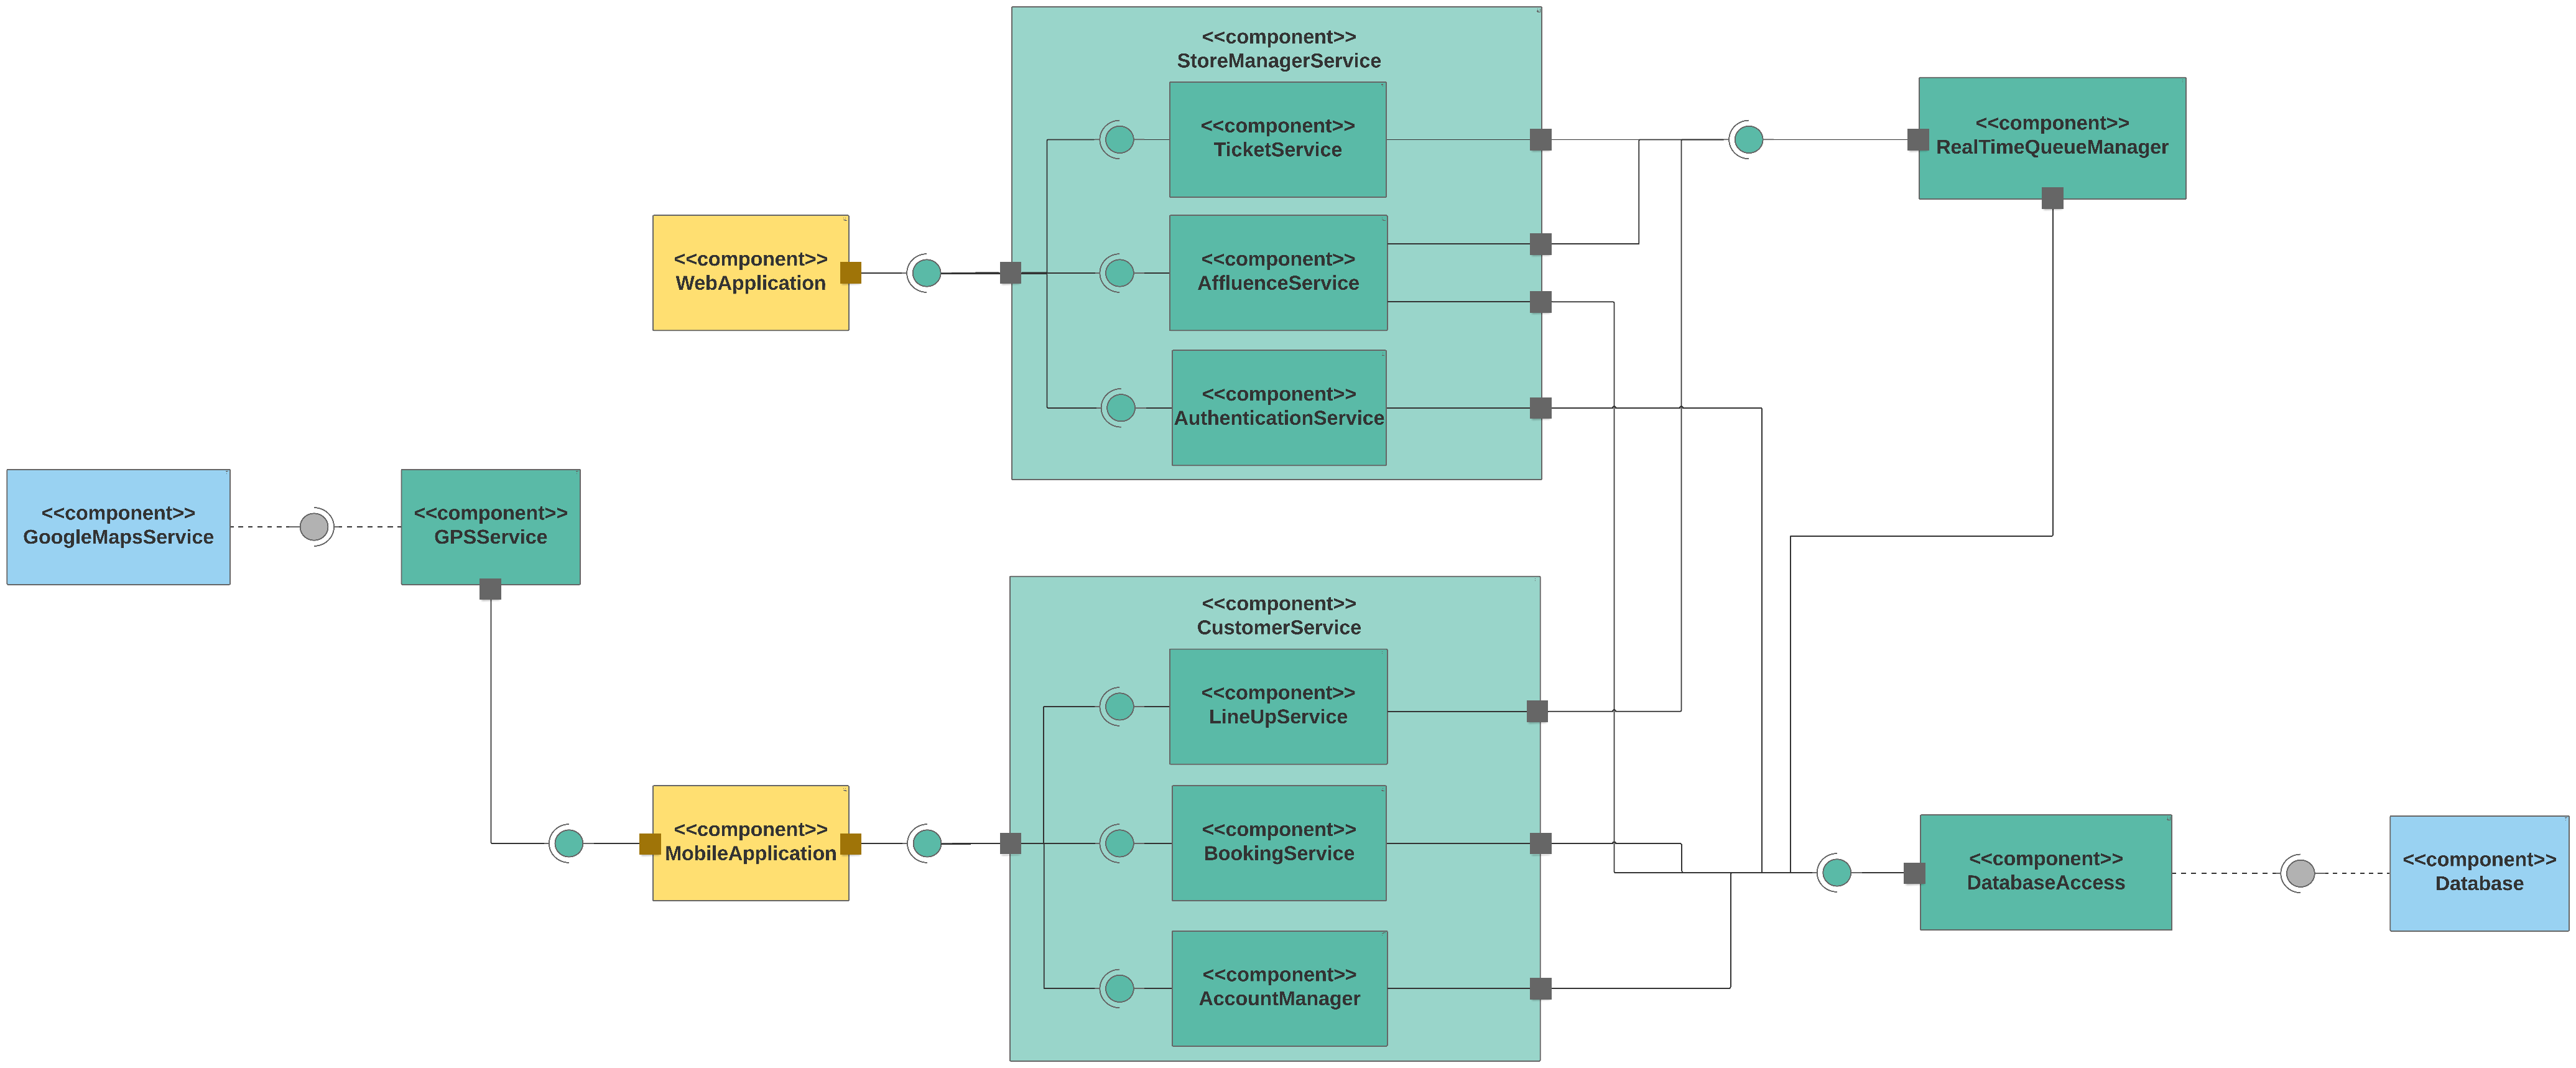
\includegraphics[scale=0.5]{./Component Diagram}}
\caption{Component Diagram}
\end{figure}



 
 